\label{sec:suspension}

%\tcb{first draft G Hammond Nov 2019}

{\bf Suspension Thermal Noise of the Mirror}
\label{sec:last_stage}

The top level requirements of a gravitational wave mirror suspension are to reduce seismic noise input from the ground and to provide a mechanism to steer the mirror via electromagnetic/electrostatic forces to enable the interferometer to be aligned and locked \emph{global control}. This must all be done while minimising the thermal noise arising from the suspension. The main components of a Virgo-like final stage are the Marionette, the Recoil Mass (RM)  and the Mirror as shown in figure \ref{LSS}. Using a VIRGO like control strategy, the marionette  ($\rm M_1$) is the first stage used to control the mirror position with coil-magnet actuators operating between the upper suspension stage and marionette arms; the recoil mass ($\rm M_3$)  is used to control Mirror ($\rm M_2$), carrying the coils of the e.m.\ actuators acting on the mirror rear side. In this section we discuss the requirements of the final stage suspension for both the Low Frequency and High frequency ET design.
\begin{figure}
    \centering
    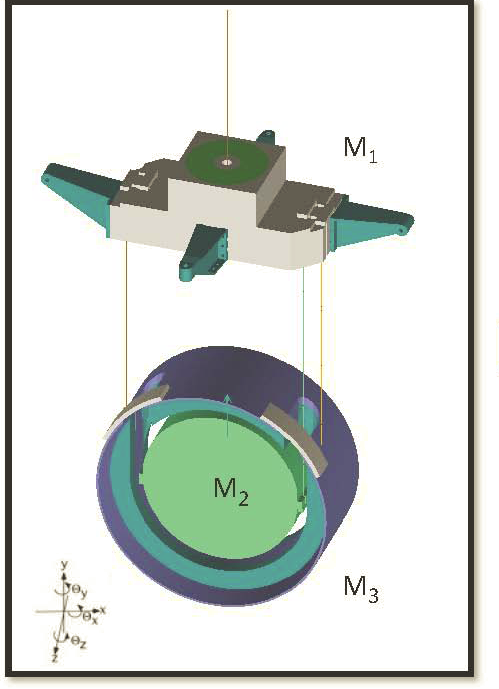
\includegraphics[width=0.35\textwidth]{./Detector/SASandSUS/SuspensionSystems/Suspension_Figures/TM_RM_M_suspension.png}
\caption{Sketch of the Virgo-like Last Stage suspension. M1:
Marionette, M2: Mirror, M3 : Recoil Mass}
    \label{LSS}
\end{figure}
Suspension thermal noise arises due to mechanical dissipation in the materials which make up the suspension (Brownian noise) or through thermoelastic noise; the coupling of statistical temperature fluctuations through the thermo-mechanical properties of the suspension materials such as the thermal expansion coefficient and the Young's modulus. The suspension thermal noise can be conveniently calculated via application of the Fluctuation-Dissipation theorem \cite{Callen:1951} which states that above the pendulum resonance the displacement thermal noise ($x_{\rm susp}$) is given by
\begin{center}
\begin{equation}\label{thermal}
x_{\rm susp}^{2}={\frac{4k_{B}T \omega_{0}^{2} \phi_{\rm total}}{m \omega^{5}}},
\end{equation}
\end{center}
where $T$ is the temperature, $m$ is the pendulum mass, $\phi_{\rm total}$ is the mechanical loss of the pendulum ($\propto 1/Q$ with Quality factor $Q$), $\omega_{0}$ is the resonant angular frequency, $k_{B}$ is Boltzmann's constant and $\omega$ is the angular frequency. The dominant contributions arise from the horizontal pendulum resonance (under 1~Hz) and the vertical bounce mode (typically 10~Hz). At higher frequencies, the violin modes also produce narrow spikes in the detector band.

A pendulum mirror suspension stores energy both in the elasticity of the fibre material and the gravitational field. The energy stored in gravity is lossless and dominates in heavily loaded suspension fibres. This implies that the pendulum loss is lower than that of the material used for the suspension fibre which is termed \emph{dissipation dilution}. The dilution allows the total mechanical loss to be diluted to $\phi_{\rm total}=\phi/D$, with $D$ being conveniently calculated from Finite Element Analysis \cite{Cumming:2009}. For aLIGO and AdVIRGO the dilution is typically 90, showing that only 2\% of energy is stored in the fused silica for the pendulum mode. For the vertical, or bounce, mode, the dilution is given by the cross coupling of the suspension. This enters through  a term due to the curvature of the Earth, and a contribution from mechanical tolerances. This is typically at the 0.1\% level.

From equation \ref{thermal}, it is clear that in order to provide low thermal displacement  noise, a combination of the heavy mirror, low mechanical loss and/or the temperature can be used to achieve the desired result. In the current ground-based room temperature, fused silica is the material of choice as its displays ultra-low mechanical loss at room tempertaure, while for KAGRA, crystalline materials (e.g. sapphire or silicon) are favoured  as they have low mechanical loss at temperatures below 150~K. These design choices, and the R\&D required will be discussed in more detail in the sections below.

{\bf High Frequency Suspension}

The current room temperature interferometers (aLIGO, AdVIRGO, GEO) utilise fused silica as a material to suspended the test masses. There is over 20 years of R\&D devoted towards ultralow noise fused silica suspension. They were initially pioneered in GEO around 1990-2000 (5.6~kg optics),  upscaled for use in aLIGO and AdVIRGO (both 40~kg optics) between 2000-2012, with installation occurring from 2015 onwards. Fused silica is the material of choice as it can be pulled into long thin fibres, can be welded to form monolithic structures, has extremely low internal friction and has a breaking strength in excess of 4~GPa. 

The dominant contributions to the mechanical loss are from;
\begin{itemize}
\item Surface loss \cite{Gretarsson:1999, Penn:2006} originates from defects on the surface such as dislocations, un-terminated dangling bonds and surface cracks. This is a dominant term for fibres which exhibit high surface to volume ratio
\item Thermoelastic loss \cite{Cagnoli:2002}, which arises from the fact that bending a suspension fibre leads to heating/cooling via the thermal expansion coefficient. When the fibre is under tension the variation in Young's modulus with temperature leads to an additional thermoelastic contribution. For fused silica these two terms have opposite sign and the thermoelastic loss can be cancelled in the bending region by suitable choice of the fibre geometry, a technique utilised in aLIGO and AdVIRGO \cite{Bell:2013}
\item Weld loss which arises from material which has been heated with a $\textrm{CO}_{2}$ laser \cite{Cumming:2012} to fuse the silica suspension fibres to the attachment ears on the side of the test mass. This material exhibits a loss which is higher than the bulk loss \cite{Heptonstall:2010} and likely correlated with the level of thermal stress. 
\item Bond loss due to the attachment of fused silica ears silicate bonded to the side of the test mass. The silicate bonding process produces a strongly cross linked structure which allows glassy materials to be reproducibly attached in a mechanically and thermally stable way \cite{Rowan:1998}. By careful suspension design this term can be minimised
\end{itemize}

The ET High Frequency suspension mirror mass will be increased to 150~kg - 200~kg to provide lower suspension thermal noise and also reduction of radiation pressure noise. There is a mature technology in place to deliver the technology for a room temperature suspension, building on many years of heritage and proven technology in the field. Material for the mirror can be sourced of sufficient quality and homogeneity using the Heraeus Suprasil family of synthetic glasses. It has already been shown that fibres of suitable geometry can be pulled and welded, and a prototype 150~kg suspension has already been demonstrated, albeit with a metal proof mass to simulate the payload. 

While current ground based detectors utilise fibres stressed to 800~Mpa in their thinnest section (to push violin modes above 500~Hz and the vertical bounce mode below 10~Hz), meeting the baseline thermal noise of ET HF further requires the fibres to be lengthened to around 1~m - 1.5~m. This has the effect of lowering the vertical bounce mode (good) and the violin modes (bad). In order to push the violin modes back up above 250~Hz will require fibres to be operated at higher stress, up to 1.2~GPa. This is the baseline proposal for the US A+ upgrade to aLIGO, and thus the ET suspension can benefit from this work also. Groups in UK and Italy are already undertaking stress corrosion tests of fibres which suggest that even at 1.2~GPa the lifetime of such fibres is greater than 1000 years \cite{Lee:2019}. Additional work has been undertaken on laser stabilisation of the fibre pulling machine which has been shown to improve the dimensional tolerance and median tensile stress of the fused silica fibres. Figure \ref{susp_thermal} shows the strain noise performance of an ET High frequency suspension with the parameters shown in table~\ref{tab:HF_params}. This comfortably meets the requirements of ET-D in the higher frequency range.

\begin{table}[h]
\begin{center}
\begin{tabular}{|p {3cm}|p{2cm}|p {3cm}|p{2cm}|} 
 \hline
 \multicolumn{4}{|c|}{ET HF Parameters} \\
 \hline
Parameter & Value & Parameter & Value   \\
 \hline
 Mass (kg)  &  150 & Length  &  1.5m  \\
 T (K) &  300  &  $r_{end}, r_{middle}$ ($\mu m$) &   762,310  \\
 $\kappa$ ($Wm^{-1}K^{-1})$ & 1.4 & C ($J kg^{-1} K^{-1})$ &  750 \\
 $h_{\phi s}$ & $4 \times 10^{-12}$ & $\phi_{weld}$   & $6\times 10^{-6}$   \\
 \hline
\end{tabular} 
\caption{Parameters used for the High Frequency suspension}
\label{tab:HF_params}
\end{center}
\end{table}


{\bf R\&D required for High Frequency Suspension}

While the fused silica solution is already well developed there needs to be work devoted towards the demonstration of a full scale ET HF prototype. Key areas of future R\&D include;
\begin{itemize}
\item A full scale prototype suspension needs to be delivered and tested. It would be sensible to consider a staged approach, whereby a full scale metal system is built first, using fused silica inserts to enable the fibres to be interfaced, ultimately leading to a fully monolithic version to test the assembly/integration/testing required. The suspension scheme proposed uses fused silica fibres with operating stresses of around 1 - 1.5~GPa, fabricated on the current fibre pulling machines cite{fibre} that have been developed for the aLIGO/AdVIRGO instruments. The fibre ends will be thickened such that they operate at a stress of 200~MPa which is needed to null the thermoelastic contribution \cite{Bell:2013}. The fibres will be welded onto "anchors/ear" using a $CO_{2}$ laser to form a system that can be integrated into the main test mass/marionette. In aLIGO, such a monolithic suspension has been shown to have extremely low mechanical losses, with quality factors for the violin modes in excess of 1 billion (a ring down of >5~days at 500~Hz).
\item Activities focused on further proving the stress-corrosion properties of fused silica, and the techniques required to bond/attach the ear/fibres to the test mass are also will naturally follow with the development of these full scale systems. Further work to ensure that the laser stabilisation techniques provide fibres of sufficient dimensional tolerance will also be useful to verify the technology.
\item The local control of test masses further plays a crucial role in gravitational wave detectors and this is an R\&D activity common to both the HF and LF suspensions. The local sensors are used to damp the suspension modes to a point at which automatic error signals (e.g. wavefront sensing for angles and locking for longitudinal position) can take over. There needs to be work to ensure there are sufficiently sensitive inertial sensors to provide the necessary performance.% (as discussed in section \ref{SAS}. 
\item Actuators also need to be developed which have suitable control bandwidth. As with aLIGO and AdVIRGO, a combination of electromagnetic voice-coil actuators at the marionette stage will be necessary to provide the control forces for large control authority local damping. Work focussing on minimising cross coupling and excess magnetic noise are necessary for a future ET HF suspension. For test ass actuation, an electrostatic actuation scheme will likely be employed, utilising high voltage actuation across the capacitance formed between the test mass and the reaction mass. R\&D to ensure that excess charging is not an issue would be an area of further research, and the current experience of discharging schemes and measurements of charge build-up in aLIGO will be helpful. 
\end{itemize}
\begin{center}
\begin{figure}
\label{strain_susp}
\caption{Strain sensitivity of the High Frequency and Low Frequency suspensions described above (need to add)}
\end{figure}
\end{center}
{\bf Low Frequency Suspension}

In addition to providing a low seismic/thermal noise platform, the ET Low Frequency suspension also has to fulfill a second crucial duty - to extract the thermal load that is put into the optical component by the laser beam. For a typical ET intra-cavity power of 18~kW and an absorption of 0.5 ppm, we may expect up to 10 milliWatts to be extracted, a challenge for operation at cryogenic temperature. In terms of material choice fused silica is ruled out both due to its low thermal conductivity, but more seriously due to the broad dissipation peak in its mechanical loss due to its amorphous nature ~\cite{McGuigan1978}. The materials of choice are crystalline materials which have a very high thermal conductivity at low temperatures and also display low mechanical loss. In particular, both silicon and sapphire are excellent materials in the temperature region of interest (typically below 20\,K). Sapphire has a higher thermal conductivity as silicon below 20\,K. Sapphire fibres for heat extraction have been investigated in detail by Japanese groups for KAGRA \cite{KAGRA:2014}~\cite{KAGRA:2016}.

At low temperatures the mechanical loss of the suspension, which defines the thermal noise performance, is a key driver for the suspension design. Again heavy test masses will be utilised, with the addition of low temperature to provide enhanced thermal noise performance. At temperature below 150~K thermoelastic noise drops away sharply, and indeed for silicon is zero around 120~K, which leaves the dominant loss mechanisms as;
\begin{itemize}
\item Surface loss \cite{Nawrodt:2013} which originates from defects on the surface such as dislocations, un-terminated dangling bonds and surface cracks. Initial measurements suggest that the surface loss at low temperature could be a factor of 10x below those of fused silica at room temperature.
\item Bond loss due to the attachment of anchors/ears via metallic or silicate bonding to the side of the test mass.
\end{itemize}
In common with the room temperature suspensions, techniques need to be developed to joint these crystalline materials Significant progress has already been made particularly for sapphire and silicon, partly due to the need of these techniques for delivering sapphire suspensions for KAGRA. There are a number of groups which have performed hydroxide-catalysis bonding of materials by growing a native oxide (e.g. wet or dry thermal oxide on silicon) or the naturally occurring oxide, and undertaking thermal cycling and mechanical loss measurements. Refs \cite{Phelps:2018b} and \cite{Haughian:2016} have shown that these bonds can be sufficiently strong and can be cycled between room temperature and cryogenic temperature. Another technique that has been explored for KAGRA is utilising metallic bonding with low temperature materials such as Indium and Gallium. This type of bonding has developed because of the need to be able to replace suspension elements. While Gallium has a much lower melting point ($\simeq$30~C), some of the challenges here are the corrosive nature and the poisonous aspects of the material, making handling a potential challenge. Indium on the other hand has a higher melting point  ($\simeq$157~C) but requires the entire suspension to be warmed to this temperature to develop strong and reproducible bonds \cite{Hofmann:2015}~\cite{Phelps:2018}. 

While sapphire is the baseline for KAGRA, the need for large and heavy test masses (150~kg - 200~kg) highlight silicon as a preferred material.  Silicon suspension elements are currently under investigation in the form of fibres~\cite{articolofibresil} and ribbon-like structures~\cite{Reid2006}. Further R\&D is focused on techniques to joint the suspension fibres to the test mass ears/anchors and this is often an overlooked but key aspect. It was noted above that the aLIGO/AdVIRGO suspensions benefit from dissipation dilution, which stores most of the fibre energy in gravity rather than elasticity. For silicon, and sapphire, suspension elements the challenge is to fabricate suspension elements that have tapered ends at the attachment points. This is essential to ensure that the bending energy of the suspension is maintained in the fibre rather than the anchor point, which will include the metallic or hydroxide catalysis bond. If this design is not carefully undertaken, the dissipation dilution of the suspension, and consequently the thermal noise performance, can be compromised. 

Currently, there are three possible techniques under investigation for the fabrication of silicon suspension elements;

\begin{itemize}
\item The micro-pulling technique~\cite{articolofibresil} where a thin fibre (diameter of up to a few millimetres) is drawn from a silicon melt through an extrusion. The fabricated fibres are not perfectly single crystalline - but recent work has improved the crystallinity of the fibres. Currently, these fibres are produces with a length of 30\,cm for the initial investigations. In principle there is no limit for the maximum achievable length and thus this technique is promising to be used for the low temperature suspensions for ET.

\item Etching suspension structures out of single crystals or wafers. This technique provides suspension elements with a rectangular cross section due to selective etching of the crystalline silicon in different directions. A number of fabrication techniques are currently under investigation including mechanical cutting, laser cutting, deep reactive ion etching and wet etching. The selective etching technique is just limited by the wafer size and in principle it is possible to create much longer elements. Current challenges are reduction in the strength of the silicon fibres due to mechanical etching, and work is underway to etch/oxidise samples to improve their strength \cite{Cumming:2014}.

\item Similar to micro-pulling, an alternative technique is to grow a fibre from a pedestal melt; so called Laser Heated Pedestal Growth. The benefit of this technique is that it can produce extremely pure fibres with high strength, as there is no interaction with a crucible or extrusion. The downside is that the production is slow (mm/min growth rate) and requires good control of temperature and growth rate. Good quality results have previously been reported by \cite{Fejer:1984} in the growth of sapphire fibres, although challenges exist with silicon as the melt changes its optical absorption strongly around the transition from solid to liquid.
\end{itemize}

Figure \ref{susp_thermal} shows the strain noise performance of an ET Low frequency suspension with the parameters shown in table \ref{LF_params}. Two temperatures have been modelled; 120~K and 20~K and the respective thermal conductivity and specific heat at these temperatures are used. The code assumes a circular fibre of equivalent cross-section to a ribbon and an idealistic dilution (this would need to be properly determined for the final geometry using FEA). Although the thermal conductivity at 120~K is poor, heat extraction would be via radiative coupling.


\begin{table}[h]
\begin{center}
\begin{tabular}{|p {3cm}|p{2cm}|p {3cm}|p{2cm}|} 
 \hline
 \multicolumn{4}{|c|}{ET LF Parameters} \\
 \hline
Parameter & Value & Parameter & Value   \\
 \hline
 Mass (kg)  &  150 & Length  &  1.5m  \\
 T (K) &  20,120  &  $r_{fibre}$ ($\mu m$) &   2200 \\
 $\kappa (120~K,20~K)$ ($Wm^{-1}K^{-1})$ & 690,4900 & C (120~K,20~K) ($J kg^{-1} K^{-1})$ &  328, 4 \\
 $h_{\phi s}$ & $5 \times 10^{-13}$ & &  \\
 \hline
\end{tabular} 
\caption{Parameters used for the Low Frequency suspension.}
\label{LF_params}
\end{center}
\end{table}


{\bf R\&D required for Low Frequency Suspension}

The cryogenic R\&D is somewhat less well developed than the room temperature approach and activities are needed on several fronts;

\begin{itemize}

\item Fibre fabrication techniques to develop long thin silicon or sapphire fibres, As noted above promising fabrication strategies include micro-pulldown, forming (etching or machining) from a wafer and laser heated pedestal growth. For all of the techniques a study of the resultant tensile strength, ease of fabrication, mechanical loss and thermomechanical properties needs to be undertaken to choose the optimum techniques. The field of micro-mechanical systems investigated surfaces losses in silicon (see e.g. \cite{Yang2000,Yasumura2000,Yang2002}). However, a systematic and general modelling of surface losses has not been made and their origin is still unclear and needs to be investigated.

\item The techniques necessary to joint suspension elements, while ensuring that dissipation dilution is maintained as high as possible, need to be properly explored. This could include hydroxide catalysis bonding of ears/anchors, metallic bonding and direct bonding techniques. Measurements of the thermal conductivity suggest that bonded silicon components at low temperature can be modelled as pure silicon with an thin ($\sim 700$ nm) interfacing glass-like layer. These results suggest that hydroxide catalysis bonding can facilitate the necessary extraction of heat, deposited on the mirrors by the incident laser beam, through to the silicon suspensions elements and towards the cooled upper-stage. A further technique worth studying is direct welding of crystalline material. Groups in UK/Italy have shown success of \emph{welding} sapphire, although this needs to be verified for silicon, and further R\&D is needed here. For example, what is the thermal conductivity of a welded joint, and does the material exhibit good thermal conductivity and low mechanical loss. 

\item A detailed FEA model of the final stage suspension needs to be undertaken in order to estimate the effects of real fibre geometries on the dissipation dilution.

\item As with the High Frequency suspension, the development of inertial sensors, with high sensitivity and large measurement band is a key point for the inertial damping to perform on the suspension system of third generation interferometric detectors. These sensors and associated actuators need to be proved for low temperature operation. There has been work proposed towards developing the monolithic folded accelerometer for cryogenic temperature \cite{Bertolini:2006}~\cite{Joris:2018}.

\item Further suspension modelling needs to be undertaken to verify the operation temperature of the Low Frequency suspension. In the previous design study an operation temperature of 10~K-20~K  was the operating point. As noted above this does result in challenges to extract sufficient heat through the suspension fibres. An alternative that surfaced in the last couple of years is the option of running close to 120~K where silicon exhibits and zero in its thermal expansion coefficient. At this temperature the thermoelastic noise is nulled and the penalty to pay is in the thermal noise performance which is roughly $\sqrt{120}{20}=2.4\times$ worse. 

\item There is a need for prototype lower stage suspension systems similar to those developed during the fused silica development era. This includes a mix of fast turnaround tabletop systems and small scale prototypes of 10m arm length with payload in the 1~kg to 10~kg range in the first instance

\end{itemize}

\begin{figure}
    \centering
    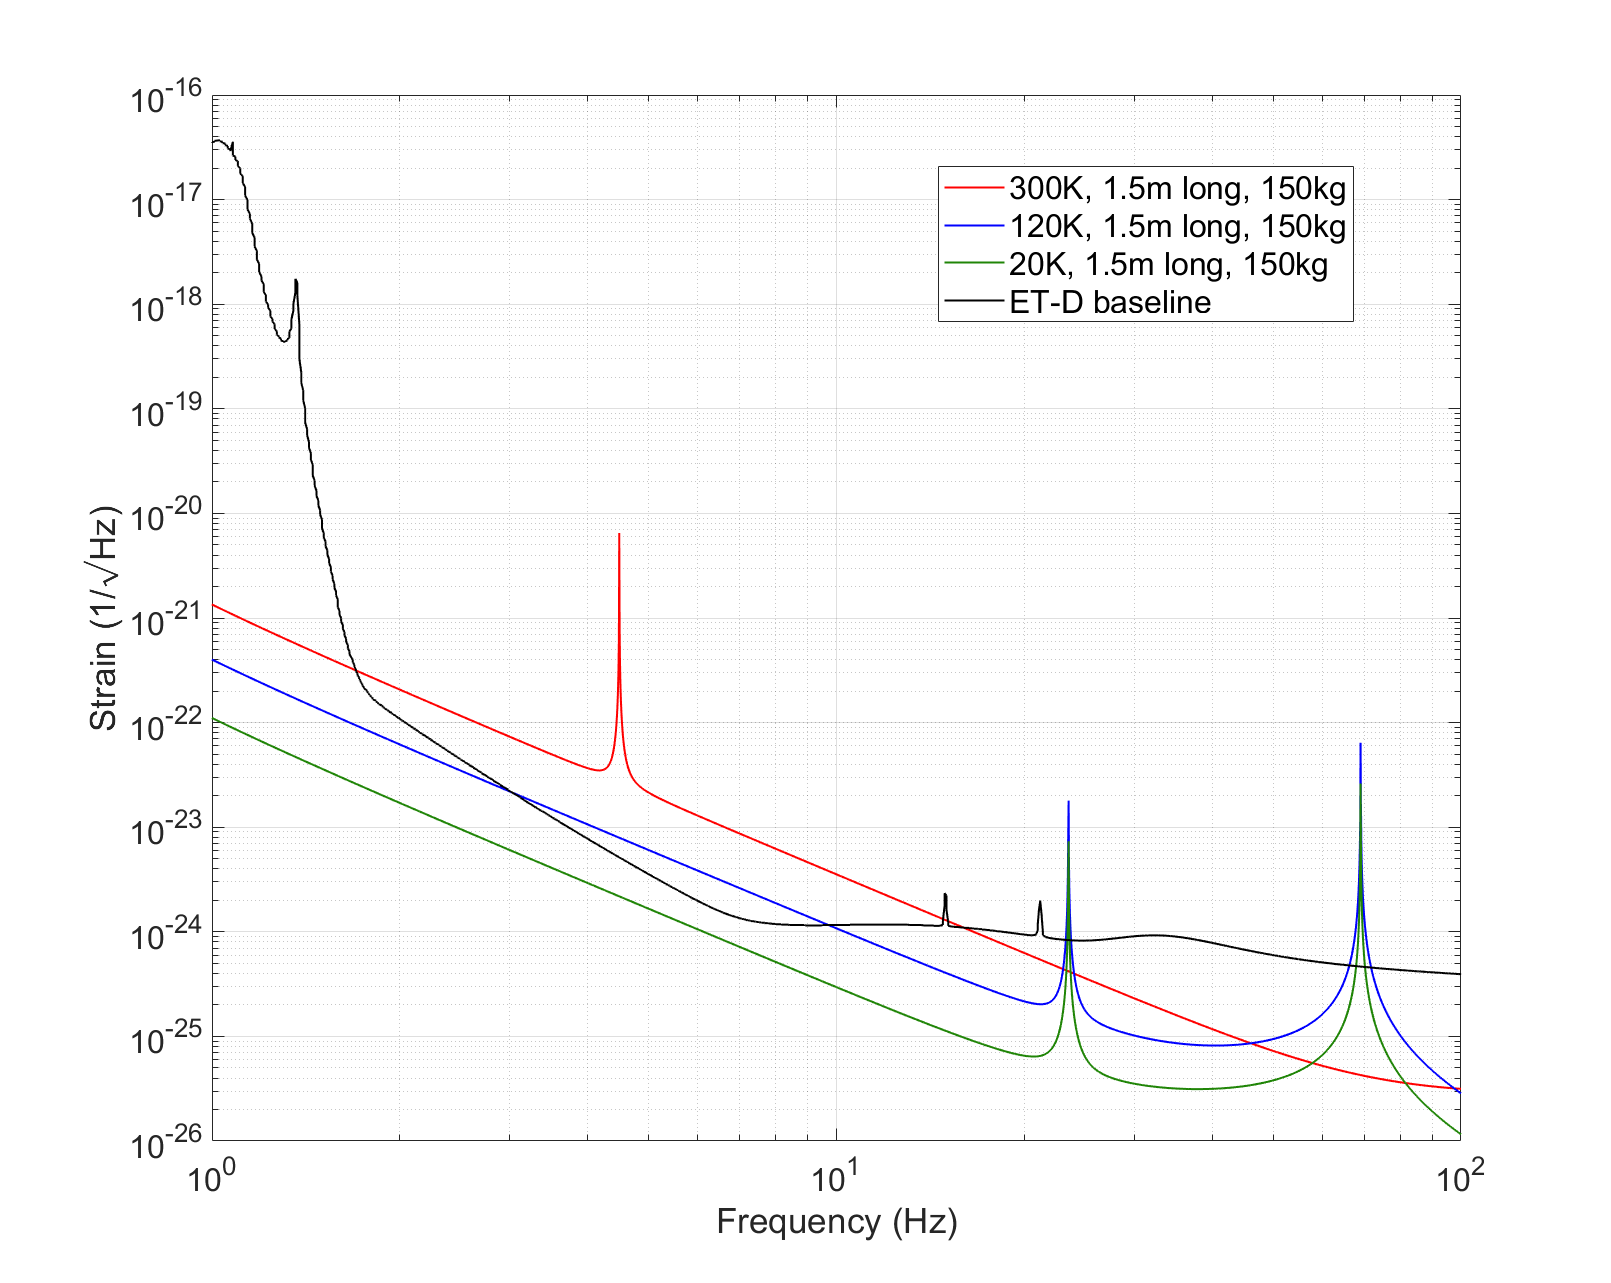
\includegraphics[width=0.8\textwidth]{./Detector/SASandSUS/SuspensionSystems/Suspension_Figures/susp_thermal.png}
\caption{Comparison of the strain sensitivity due to suspension thermal noise for the configurations described above; red: room temperature silica, blue 120~K silicon, green 20~K silicon, black ET-D baseline}
    \label{susp_thermal}
\end{figure}

